\chapter{Swaps and Bootstrapping}\label{swaps-and-bootstrapping---practical-lesson-5}

In this Chapter the Overnight Index Swap contract is reviewed and a new class to represent 
will be added to our financial module. Beside financial arguments another very important mathematical technique is introduced: the \emph{bootstrapping}.

\section{Payment Dates Generator}
Before going to describe the Overnight Index Swap we need to develop a tool which helps us to generate list of dates (e.g. payment dates), a task that we need to do often from now on. 
The function we are writing will go in \texttt{finmarkets} module and will be used by the classes describing various kind of contracts.

\begin{tcolorbox}[size=fbox, boxrule=1pt, colback=cellbackground, colframe=cellborder]
\begin{Verbatim}[commandchars=\\\{\}]
\PY{k+kn}{from} \PY{n+nn}{datetime} \PY{k}{import} \PY{n}{date}
\PY{k+kn}{from} \PY{n+nn}{dateutil}\PY{n+nn}{.}\PY{n+nn}{relativedelta} \PY{k}{import} \PY{n}{relativedelta}

\PY{k}{def} \PY{n+nf}{generate\PYZus{}swap\PYZus{}dates}\PY{p}{(}\PY{n}{start\PYZus{}date}\PY{p}{,} \PY{n}{n\PYZus{}months}\PY{p}{)}\PY{p}{:}
    \PY{n}{dates} \PY{o}{=} \PY{p}{[}\PY{p}{]}
    \PY{k}{for} \PY{n}{i} \PY{o+ow}{in} \PY{n+nb}{range}\PY{p}{(}\PY{l+m+mi}{0}\PY{p}{,} \PY{n}{n\PYZus{}months}\PY{p}{,} \PY{l+m+mi}{12}\PY{p}{)}\PY{p}{:}
        \PY{n}{dates}\PY{o}{.}\PY{n}{append}\PY{p}{(}\PY{n}{start\PYZus{}date} \PY{o}{+} \PY{n}{relativedelta}\PY{p}{(}\PY{n}{months}\PY{o}{=}\PY{n}{i}\PY{p}{)}\PY{p}{)}
    \PY{n}{dates}\PY{o}{.}\PY{n}{append}\PY{p}{(}\PY{n}{start\PYZus{}date} \PY{o}{+} \PY{n}{relativedelta}\PY{p}{(}\PY{n}{months}\PY{o}{=}\PY{n}{n\PYZus{}months}\PY{p}{)}\PY{p}{)}
    
    \PY{k}{return} \PY{n}{dates}

\PY{n+nb}{print} \PY{p}{(}\PY{n}{generate\PYZus{}swap\PYZus{}dates}\PY{p}{(}\PY{n}{date}\PY{o}{.}\PY{n}{today}\PY{p}{(}\PY{p}{)}\PY{p}{,} \PY{l+m+mi}{25}\PY{p}{)}\PY{p}{)}

[datetime.date(2020, 10, 20), datetime.date(2021, 10, 20), datetime.date(2022,
10, 20), datetime.date(2022, 11, 20)]
    \end{Verbatim}
\end{tcolorbox}

\section{Overnight Index Swap}\label{overnight-index-swap}

Interest rate swaps (IRS) are generally used to mitigate the risks of
fluctuations of varying interest rates, or to benefit from lower rates.

Overnight Index Swaps (OIS) are a particular kind of IRS which pay a
floating coupon, determined by overnight rate fixings over the reference
periods, against a fixed coupon. By definition an OIS is defined by:

\begin{itemize}
\tightlist
\item
  a notional amount \(N\);
\item
  a starting date \(d_0\);
\item
  a sequence of payment dates \(d_1,...,d_n\);
\item
  a fixed rate \(K\).
\end{itemize}

For simplicity in the following we are assuming that the fixed and
floating legs of our OIS have the same notional and payment dates,
although this is not necessarily always the case in practice.
We will always look at these products from the point of view of the
\textbf{receiver of the floating leg}.

\subsection{OIS Valuation}\label{ois-valuation}
To evaluate the net present value (NPV) of such products the cash flows
of each leg have to be calculated; today's NPV then is the sum of all
the discounted cash flows.

\subsubsection{Floating leg}\label{floating-leg}

At each payment date, the floating leg pays a cash flow determined as
follows:

\begin{equation}
f_{\mathrm{float},~i} = N \Bigg\{\prod_{d=d_{i-1}}^{d=d_i-1}\Big(1+r_{\mathrm{O/N}}(d)\cdot\frac{1}{360}\Big) -1 \Bigg\}
\label{eq:floati_ois}
\end{equation}

Strictly speaking this formula is valid for an EONIA swaps
(i.e.\textasciitilde{}for OIS swaps in EUR) other currencies might have
different conventions. The \(\frac{1}{360}\) fraction appears because
EONIA rates are quoted using the ACT/360 day-count convention. In
addition we are making the simplifying assumption of ignoring weekends
and holidays, so we assume that each overnight rate is valid for only
one day. The sum of the discounted expected values of these cash flows
is

\begin{equation}
\mathrm{NPV}_{\mathrm{float}} = \sum_{i=1}^{n}D(d_i)\mathbb{E}[f_{\mathrm{float},~i}]
\end{equation}
where \(D(d)\) is the discount factor with expiry \(d\). On the other
hand we have seen from the forward rate definition (see Section~\ref{calculating-forward-rates}) that

\begin{equation*}
\underbrace{(1+r_{0,1}\Delta T)\underbrace{(1+r_{1,2}\Delta T)\ldots\underbrace{(1+r_{d-2,d-1}\Delta T)(1+r_{d-1,d}\Delta T)}_{=(1+r_{d-2,d}\Delta T)}}_{=(1+r_{1,d}\Delta T)}}_{=(1+r_{0,d}\Delta T)}
\end{equation*}
So the product in Eq.~\ref{eq:floating_ois} can be simplified into

\begin{equation}
\mathbb{E}[f_{\mathrm{float},~i}] = N\cdot\Big(\frac{D_{\mathrm{OIS}}(d_{i-1})}{D_{\mathrm{OIS}}(d_{i})} - 1\Big)
\end{equation}
hence
\begin{equation}
\mathrm{NPV}_{\mathrm{float}} = N\cdot \sum_{i=1}^{n}D(d_i) \Big(\frac{D_{\mathrm{OIS}}(d_{i-1})}{D_{\mathrm{OIS}}(d_{i})} - 1\Big)
\end{equation}
where \(D_{\mathrm{OIS}}(d)\) is the discount factor implied by OIS
prices (we will see how to derive it).

%The correct curve to use for discounting the flows of a collateralized contract, like OIS, is the one associated with the collateral. Since OIS contracts are collateralized with cash, and cash accrues daily interest at the overnight rate, the OIS curve is itself the correct curve with which to discount the flows of an OIS contract ! 
%From what has been said in Section~\ref{sec:financial-crisis}
%Since the financial crisis, in the Euro area the rates used for
%discounting has been the EONIA rates. Similarly, in other jurisdictions
%it has been used other overnight rates such us Fed fund rates in USA.
%This practice is consistent with the daily remuneration of the
%collateral (i.e. cash given or received as mitigants for credit risk
%arising from the mark to market of the derivatives contract).
%For arbitrage consideration the discounting curve of future cash flows
%in a derivative contract can only be the one derived from the rates
%applied for the collateral.
%
%So we have that \(D = D_{\mathrm{OIS}}\) and the NPV simplifies to

From what has been said in Section~\ref{sec:financial-crisis} we have that 
\(D = D_{\mathrm{OIS}}\) and the NPV simplifies to

\begin{equation}
  \begin{split}
    \mathrm{NPV}_{\mathrm{float}} & = N\cdot\sum_{i=1}^{n}[D(d_{i-1}) - D(d_i)] =  \\
    &= N\cdot[(D(d_{0}) - D(d_{1})) + (D(d_{1}) - D(d_{2})) + ... + (D(d_{n-1}) - D(d_{n}))]\\
    &= N \cdot [D(d_0) - D(d_n)]
  \end{split}
\end{equation}

\subsubsection{Fixed leg}\label{fixed-leg}

The calculation for the fixed leg is simpler; each cash flow is equal to

\begin{equation}
f_{\mathrm{fixed},~i}=N\cdot K\cdot \frac{d_i - d_{i-1}}{360}
\end{equation}
so the NPV of the fixed leg is

\begin{equation}
\mathrm{NPV}_{\mathrm{fixed}} = N\cdot K\cdot \sum_{i=1}^{n}D(d_{i})\frac{d_i - d_{i-1}}{360}
\end{equation}

\subsection{\texttt{OvernightIndexSwap} Class}\label{discount-factor-determination-from-market-quotes}

Our ultimate goal is to take a series of Overnight Index Swap
quotations, and determine the discount factors implied by their prices.
To do this we will build a class to represent OIS and compute its value,
given a particular discount curve. Then we will use this class, put inside
a numerical optimizer, to \emph{invert} the relationship that connects 
NPV and discount curve so that the \emph{implied} discount
factors can be determined from OIS market quotes.

\begin{tcolorbox}[breakable, size=fbox, boxrule=1pt, pad at break*=1mm,colback=cellbackground, colframe=cellborder]
\begin{Verbatim}[commandchars=\\\{\}]
\PY{k}{class} \PY{n+nc}{OvernightIndexSwap}\PY{p}{:}
    \PY{k}{def} \PY{n+nf}{\PYZus{}\PYZus{}init\PYZus{}\PYZus{}}\PY{p}{(}\PY{n+nb+bp}{self}\PY{p}{,} \PY{n}{notional}\PY{p}{,} \PY{n}{payment\PYZus{}dates}\PY{p}{,} \PY{n}{fixed\PYZus{}rate}\PY{p}{)}\PY{p}{:}
        \PY{n+nb+bp}{self}\PY{o}{.}\PY{n}{notional} \PY{o}{=} \PY{n}{notional}
        \PY{n+nb+bp}{self}\PY{o}{.}\PY{n}{payment\PYZus{}dates} \PY{o}{=} \PY{n}{payment\PYZus{}dates}
        \PY{n+nb+bp}{self}\PY{o}{.}\PY{n}{fixed\PYZus{}rate} \PY{o}{=} \PY{n}{fixed\PYZus{}rate}

    \PY{k}{def} \PY{n+nf}{npv\PYZus{}floating\PYZus{}leg}\PY{p}{(}\PY{n+nb+bp}{self}\PY{p}{,} \PY{n}{discount\PYZus{}curve}\PY{p}{)}\PY{p}{:}
        \PY{k}{return} \PY{n+nb+bp}{self}\PY{o}{.}\PY{n}{notional} \PY{o}{*} \PY{p}{(}\PY{n}{discount\PYZus{}curve}\PY{o}{.}\PY{n}{df}\PY{p}{(}\PY{n+nb+bp}{self}\PY{o}{.}\PY{n}{payment\PYZus{}dates}\PY{p}{[}\PY{l+m+mi}{0}\PY{p}{]}\PY{p}{)} \PY{o}{\PYZhy{}}
               \PY{n}{discount\PYZus{}curve}\PY{o}{.}\PY{n}{df}\PY{p}{(}\PY{n+nb+bp}{self}\PY{o}{.}\PY{n}{payment\PYZus{}dates}\PY{p}{[}\PY{o}{\PYZhy{}}\PY{l+m+mi}{1}\PY{p}{]}\PY{p}{)}\PY{p}{)}

    \PY{k}{def} \PY{n+nf}{npv\PYZus{}fixed\PYZus{}leg}\PY{p}{(}\PY{n+nb+bp}{self}\PY{p}{,} \PY{n}{discount\PYZus{}curve}\PY{p}{)}\PY{p}{:}
        \PY{n}{npv} \PY{o}{=} \PY{l+m+mi}{0}
        \PY{k}{for} \PY{n}{i} \PY{o+ow}{in} \PY{n+nb}{range}\PY{p}{(}\PY{l+m+mi}{1}\PY{p}{,} \PY{n+nb}{len}\PY{p}{(}\PY{n+nb+bp}{self}\PY{o}{.}\PY{n}{payment\PYZus{}dates}\PY{p}{)}\PY{p}{)}\PY{p}{:}
            \PY{n}{start\PYZus{}date} \PY{o}{=} \PY{n+nb+bp}{self}\PY{o}{.}\PY{n}{payment\PYZus{}dates}\PY{p}{[}\PY{n}{i}\PY{o}{\PYZhy{}}\PY{l+m+mi}{1}\PY{p}{]}
            \PY{n}{end\PYZus{}date} \PY{o}{=} \PY{n+nb+bp}{self}\PY{o}{.}\PY{n}{payment\PYZus{}dates}\PY{p}{[}\PY{n}{i}\PY{p}{]}
            \PY{n}{tau} \PY{o}{=} \PY{p}{(}\PY{n}{end\PYZus{}date} \PY{o}{\PYZhy{}} \PY{n}{start\PYZus{}date}\PY{p}{)}\PY{o}{.}\PY{n}{days} \PY{o}{/} \PY{l+m+mi}{360}
            \PY{n}{df} \PY{o}{=} \PY{n}{discount\PYZus{}curve}\PY{o}{.}\PY{n}{df}\PY{p}{(}\PY{n}{end\PYZus{}date}\PY{p}{)}
            \PY{n}{npv} \PY{o}{=} \PY{n}{npv} \PY{o}{+} \PY{n}{df} \PY{o}{*} \PY{n}{tau}
        \PY{k}{return} \PY{n+nb+bp}{self}\PY{o}{.}\PY{n}{notional} \PY{o}{*} \PY{n+nb+bp}{self}\PY{o}{.}\PY{n}{fixed\PYZus{}rate} \PY{o}{*} \PY{n}{npv}
    \PY{k}{def} \PY{n+nf}{npv}\PY{p}{(}\PY{n+nb+bp}{self}\PY{p}{,} \PY{n}{discount\PYZus{}curve}\PY{p}{)}\PY{p}{:}
        \PY{n}{float\PYZus{}npv} \PY{o}{=} \PY{n+nb+bp}{self}\PY{o}{.}\PY{n}{npv\PYZus{}floating\PYZus{}leg}\PY{p}{(}\PY{n}{discount\PYZus{}curve}\PY{p}{)}
        \PY{n}{fixed\PYZus{}npv} \PY{o}{=} \PY{n+nb+bp}{self}\PY{o}{.}\PY{n}{npv\PYZus{}fixed\PYZus{}leg}\PY{p}{(}\PY{n}{discount\PYZus{}curve}\PY{p}{)}
        \PY{k}{return} \PY{n}{float\PYZus{}npv} \PY{o}{\PYZhy{}} \PY{n}{fixed\PYZus{}npv}
\end{Verbatim}
\end{tcolorbox}

To test the newly developed class we need a discount curve. In the
following example a fake curve will be defined, and then used with an
OIS product.

\begin{tcolorbox}[breakable, size=fbox, boxrule=1pt, pad at break*=1mm,colback=cellbackground, colframe=cellborder]
\begin{Verbatim}[commandchars=\\\{\}]
\PY{k+kn}{from} \PY{n+nn}{datetime} \PY{k}{import} \PY{n}{date}
\PY{k+kn}{from} \PY{n+nn}{finmarkets} \PY{k}{import} \PY{n}{DiscountCurve}

\PY{n}{ois} \PY{o}{=} \PY{n}{OvernightIndexSwap}\PY{p}{(}
            \PY{c+c1}{\PYZsh{} the notional, one million}
            \PY{l+m+mf}{1e6}\PY{p}{,}
            \PY{c+c1}{\PYZsh{} the list of product dates,}
            \PY{c+c1}{\PYZsh{} i.e. the start date then the payment dates}
            \PY{p}{[}\PY{n}{date}\PY{p}{(}\PY{l+m+mi}{2020}\PY{p}{,} \PY{l+m+mi}{1}\PY{p}{,} \PY{l+m+mi}{1}\PY{p}{)}\PY{p}{,} \PY{n}{date}\PY{p}{(}\PY{l+m+mi}{2020}\PY{p}{,} \PY{l+m+mi}{4}\PY{p}{,} \PY{l+m+mi}{1}\PY{p}{)}\PY{p}{,}
             \PY{n}{date}\PY{p}{(}\PY{l+m+mi}{2020}\PY{p}{,} \PY{l+m+mi}{7}\PY{p}{,} \PY{l+m+mi}{1}\PY{p}{)}\PY{p}{,} \PY{n}{date}\PY{p}{(}\PY{l+m+mi}{2020}\PY{p}{,} \PY{l+m+mi}{10}\PY{p}{,} \PY{l+m+mi}{1}\PY{p}{)}\PY{p}{,}
             \PY{n}{date}\PY{p}{(}\PY{l+m+mi}{2021}\PY{p}{,} \PY{l+m+mi}{1}\PY{p}{,} \PY{l+m+mi}{1}\PY{p}{)}\PY{p}{]}\PY{p}{,}
            \PY{c+c1}{\PYZsh{} the fixed rate, 2.5\PYZpc{}}
            \PY{l+m+mf}{0.025}\PY{p}{)}

\PY{n}{curve} \PY{o}{=} \PY{n}{DiscountCurve}\PY{p}{(}\PY{n}{date}\PY{p}{(}\PY{l+m+mi}{2020}\PY{p}{,} \PY{l+m+mi}{1}\PY{p}{,} \PY{l+m+mi}{1}\PY{p}{)}\PY{p}{,}
                      \PY{p}{[}\PY{n}{date}\PY{p}{(}\PY{l+m+mi}{2020}\PY{p}{,} \PY{l+m+mi}{1}\PY{p}{,} \PY{l+m+mi}{1}\PY{p}{)}\PY{p}{,} \PY{n}{date}\PY{p}{(}\PY{l+m+mi}{2021}\PY{p}{,} \PY{l+m+mi}{6}\PY{p}{,} \PY{l+m+mi}{1}\PY{p}{)}\PY{p}{,}
                       \PY{n}{date}\PY{p}{(}\PY{l+m+mi}{2022}\PY{p}{,} \PY{l+m+mi}{1}\PY{p}{,} \PY{l+m+mi}{1}\PY{p}{)}\PY{p}{]}\PY{p}{,}
                      \PY{p}{[}\PY{l+m+mf}{1.0}\PY{p}{,} \PY{l+m+mf}{0.98}\PY{p}{,} \PY{l+m+mf}{0.82}\PY{p}{]}\PY{p}{)}

\PY{n}{ois}\PY{o}{.}\PY{n}{npv}\PY{p}{(}\PY{n}{curve}\PY{p}{)}

105332.192377
\end{Verbatim}
\end{tcolorbox}

\section{Bootstrap Technique}\label{bootstrapping-technique}

As we said before we would like to determine a \emph{real} discount
curve starting from the market quotes of a set of Overnight Index Swaps
with different maturities, this will be done via a technique called
bootstrapping. It is the ABC of financial mathematics, since you
always need a discount curve to price a contract. We are
going to concentrate on EONIA swaps in order to build an EUR discount
curve.

\subsection{Building OIS Instances}
\label{building-ois-instances}

The first step involves getting data, the swap market quotes, and this is not actually as simple as it sounds.

The issue is that EONIA swap market is over the counter (OTC) and it's not straightforward to access it. Unlike (some) listed futures, where anyone with a retail brokerage account can view and apply real time prices, to trade in the EONIA swap market you have to be a financial institution or at least a large company and have an agreement with a broker which operates in the market. One of the main brokers in the OIS market is ICAP, see Fig.~\ref{fig:icap}.

\begin{figure}[bth]
  \centering
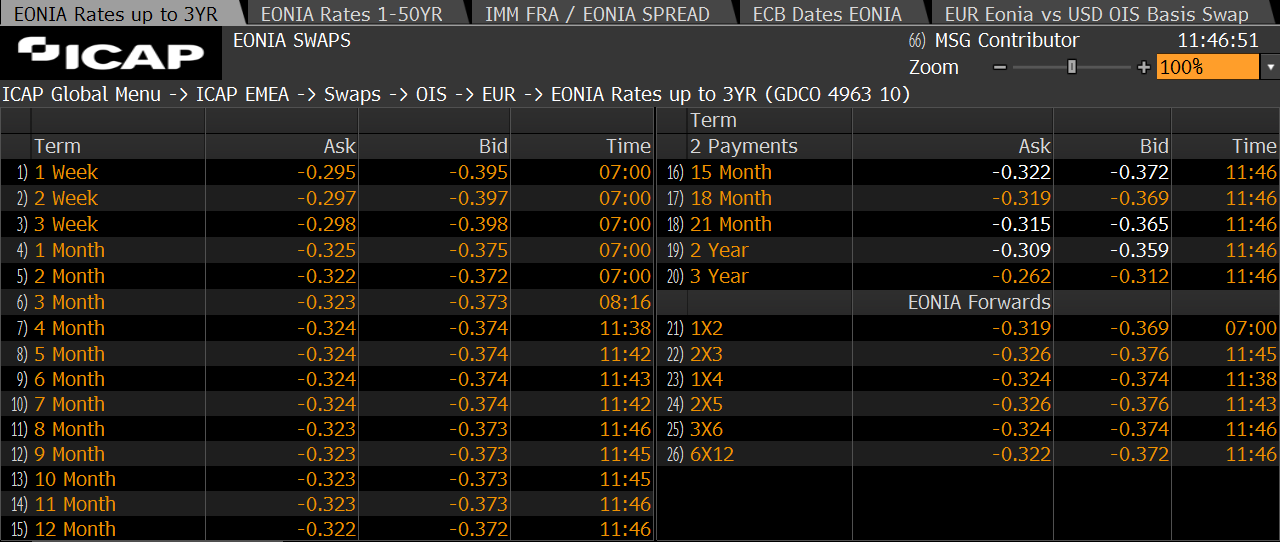
\includegraphics[width=1.\linewidth]{figures/icap_3.png}
\caption{Screenshot of market quotes from ICAP.}
\label{fig:icap}
\end{figure}

Though there exist some electronic platform in which market participants post bids and offers and other participants can apply them, in practice a lot of trading is still done over "voice", i.e.~by phone or more
commonly over chat. For convenience, however, Bloomberg provides a service which displays indicative real time rates as provided by a selection of relevant brokers (\emph{interest rate swap quotes vary from standard price quotes of commonly traded instruments, they can appear puzzling because the quotes are effectively interest rates}).

In the following we use a similarly created data-set (\href{https://drive.google.com/file/d/1LCEDmheKqwPXFpJ25hFz32QI5im2UJO1/view?usp=sharing}{\texttt{ois\_data.xlsx}}) to derive our discount curve; with the help of \texttt{pandas} the data-set can be inspected:

\begin{tcolorbox}[breakable, size=fbox, boxrule=1pt, pad at break*=1mm,colback=cellbackground, colframe=cellborder]
\begin{Verbatim}[commandchars=\\\{\}]
\PY{k+kn}{import} \PY{n+nn}{pandas}\PY{o}{,} \PY{n+nn}{datetime}

\PY{n}{observation\PYZus{}date} \PY{o}{=} \PY{n}{datetime}\PY{o}{.}\PY{n}{date}\PY{o}{.}\PY{n}{today}\PY{p}{(}\PY{p}{)}

\PY{n}{mq} \PY{o}{=} \PY{n}{pandas}\PY{o}{.}\PY{n}{read\PYZus{}csv}\PY{p}{(}\PY{l+s+s1}{\PYZsq{}}\PY{l+s+s1}{ois\PYZus{}data.csv}\PY{l+s+s1}{\PYZsq{}}\PY{p}{)}
\PY{n}{mq}\PY{o}{.}\PY{n}{head}\PY{p}{(}\PY{p}{)}

   months  quote
0       1 -0.350
1       2 -0.347
2       3 -0.348
3       4 -0.350
4       5 -0.350
\end{Verbatim}
\end{tcolorbox}
\noindent
Next we could convert the data-set into a dictionary for later usage or
use the \(\tt{DataFrame}\) directly, it is just matter of taste.

Let's say we want to build a 15 months swap instance using data
contained in \(\tt{ois\_data}\) file. Be careful when doing this
operation and double check the units of rates, quotes\ldots in
this case for example quotes are expressed in percent so you need to
multiply them by 0.01 before using them. Another detail to check is that
15 months quote is not the fifteenth entry in the \(\tt{DataFrame}\)
(actually it is the twelfth).

\begin{tcolorbox}[breakable, size=fbox, boxrule=1pt, pad at break*=1mm, colback=cellbackground, colframe=cellborder]
\begin{Verbatim}[commandchars=\\\{\}]
\PY{n}{ois} \PY{o}{=} \PY{n}{OvernightIndexSwap}\PY{p}{(}\PY{l+m+mf}{1e6}\PY{p}{,}
                         \PY{p}{[}\PY{n}{date}\PY{p}{(}\PY{l+m+mi}{2019}\PY{p}{,} \PY{l+m+mi}{10}\PY{p}{,} \PY{l+m+mi}{23}\PY{p}{)}\PY{p}{,} \PY{n}{date}\PY{p}{(}\PY{l+m+mi}{2020}\PY{p}{,} \PY{l+m+mi}{10}\PY{p}{,} \PY{l+m+mi}{23}\PY{p}{)}\PY{p}{,}
                          \PY{n}{date}\PY{p}{(}\PY{l+m+mi}{2020}\PY{p}{,} \PY{l+m+mi}{1}\PY{p}{,} \PY{l+m+mi}{23}\PY{p}{)}\PY{p}{]}\PY{p}{,}
                         \PY{n}{mq}\PY{p}{[}\PY{l+s+s1}{\PYZsq{}}\PY{l+s+s1}{quote}\PY{l+s+s1}{\PYZsq{}}\PY{p}{]}\PY{o}{.}\PY{n}{tolist}\PY{p}{(}\PY{p}{)}\PY{p}{[}\PY{l+m+mi}{12}\PY{p}{]}\PY{o}{*}\PY{l+m+mf}{0.01}\PY{p}{)}

\PY{n}{ois}\PY{o}{.}\PY{n}{payment\PYZus{}dates}\PY{p}{[}\PY{o}{\PYZhy{}}\PY{l+m+mi}{1}\PY{p}{]}

datetime.date(2020, 1, 23)
\end{Verbatim}
\end{tcolorbox}

Clearly to use the \texttt{npv} method to calculate the OIS' NPV we need a discount curve with which to evaluate it and here comes to hand the bootstrapping technique !

\subsection{Constructing the Yield Curve}\label{the-bootstrapping-technique}

Keep aside for a moment our swaps and introduce the \emph{bootstrap
algorithm}. In finance, bootstrapping is a method for constructing a
(zero-coupon) fixed-income yield curve from the prices of a set of
coupon-bearing products, e.g. bonds and swaps. The term structure of
spot returns is obtained from the bond yields by solving for them
recursively, by forward substitution: this iterative process is what is
called the bootstrap method. The usefulness of bootstrap is that using
only a few carefully selected zero-coupon products, it becomes possible
to derive swap forward and spot rates for all maturities given the
solved curve.

The underlying assumption is that market quotes represent the \textbf{fair price} of 
the contracts so they make the theis NPVs null (the fair price is an estimate of what 
a willing buyer would pay a willing seller for a given asset, assuming both have 
a reasonable knowledge of the asset's worth).

To illustrate bootstrapping let's consider the following example which can be partially solved analytically: we have some coupon paying bond (coupons of 4\%, 5\%, 6\%, 7\% and 8\% respectively) with maturities ranging from 1 to 5 years, each having a value of \euro{100} and traded at par. To determine the zero-coupon yield curve proceed as follows:
\begin{enumerate}
\item at the end of the first year the $1^{st}$ bond will pay a coupon of \euro{4} (= \euro{100} * 4\%) plus the principal amount (= \euro{100}) which sums up to \euro{104} while the bond is trading at \euro{100}. Therefore, the implied 1-year spot \emph{fair} rate $S_{1y}$ can be calculated as, $\mbox{\euro{100}} = \mbox{\euro{104}} / (1 + S_{1y})$;

\item at the end of second year the sum of the cash flows of the $2^{nd}$ bond can be compared to its trading price to compute the 2-year spot rate $S_{2y}$ as $\mbox{\euro{100}} = \mbox{\euro{5}} / (1 + S_{1y}) + \mbox{\euro{105}} / (1 + S_{2y})^{2}$ where the previously derived value of $S_{1y}$ is used;

\item at the end of third year the sum of the cash flows of the $3^{rd}$ bond can be compared to its trading price to calculate the 3-year spot rate $S_{3y}$ as $\mbox{\euro{100}} = \mbox{\euro{6}} / (1 + S_{1y}) + \mbox{\euro{6}} / (1 + S_{2y})^{2} + \mbox{\euro{106}} / (1 + S_{3y})^{3}$, using $S_{1y}$ and $S_{2y}$ computed before;

\item and so on for the other bonds\ldots
\end{enumerate}

Putting all together we can construct a system of equations (now omitting the currency symbol for simplicity):

\begin{equation}
\begin{cases}
100 = \cfrac{104}{(1 + S_{1y})} \\
100 = \cfrac{5}{(1 + S_{1y})} + \cfrac{105}{(1 + S_{2y})^{2}} \\
100 = \cfrac{6} {(1 + S_{1y})} + \cfrac{6}{(1 + S_{2y})^{2}} + \cfrac{106} {(1 + S_{3y})^{3}} \\
100 = \cfrac{7} {(1 + S_{1y})} + \cfrac{7} {(1 + S_{2y})^{2}} + \cfrac{7} {(1 + S_{3y})^{3}} + \cfrac{107} {(1 + S_{4y})^{4}} \\
100 = \cfrac{8} {(1 + S_{1y})} + \cfrac{8} {(1 + S_{2y})^{2}}+ \cfrac{8} {(1 + S_{3y})^{3}} + \cfrac{8} {(1 + S_{4y})^{4}} + \cfrac{108} {(1 + S_{5y})^{5}}
\end{cases}
\label{eq:fifth_year_rate}
\end{equation}

This system can be solved quite easily: $S_{1y}$ can be derived from the first equation, $S_{2y}$ from the second, $S_{3y}$ from the third, \ldots. So

\begin{equation}
100 = 104 / (1 + S_{1y})\quad\Rightarrow\quad S_{1y} = 104/100 - 1 = 4\%
\end{equation}
Moving to the second equation:
\begin{equation}
\begin{split}
& 100 = 5 / (1 + 0.04) + 105 / (1 + S_{2y})^{2}\quad\Rightarrow\quad S_{2y}^2  + 2 S_{2y}  - 0.103030 = 0 \\
& S_{2y} = - 1 \pm \sqrt{1 + 0.103030} = \begin{cases}\text{\sout{-2.05023}} \\ 0.0503\end{cases}
\end{split}
\end{equation}
where the first solution has been discarded because negative.

From the third on it is not as simple to solve them analytically since they involve third order (or more) equations, anyway it is possible to solve them numerically.
Assume we have found all the rates up to the fourth year (they are reported in Table~\ref{tab:rates}) and let's try to determine the last one.

\begin{table}[htb]
\begin{center}
\begin{tabular}{|c|c|c|c|}
\hline
\textbf{years} & \textbf{coupon rate} & \textbf{bond price} & \textbf{spot rate} \\
\hline
1 & 1.00 \% & \euro{100} & 4.00\% \\
\hline
2 & 2.00 \% & \euro{100} & 5.03\% \\
\hline
3 & 3.00 \% & \euro{100} & 6.08\% \\
\hline
4 & 4.00 \% & \euro{100} & 7.19\% \\
\hline
5 & 5.00 \% & \euro{100} & ??? \\
\hline
\end{tabular}
\end{center}
\caption{Table reporting maturity, coupon, bond price and implied spot rate for the example outlined in the text.}
\label{tab:rates}
\end{table}
The last column of Table~\ref{tab:rates} provides the terms to fill the zero-coupon yield curve.
To solve the last equation numerically we can use \texttt{scipy.optimize.brentq} algorithm which finds zeros of a user-defined function given a validity interval.
In Figure~\ref{fig:fifth_year_rate} the function to determine the 5 year rate expressed in the last of Eqs.~\ref{eq:fifth_year_rate} is shown. From the plot we expect the rate to be around 0.08.

\begin{figure}[htb]
  \centering
  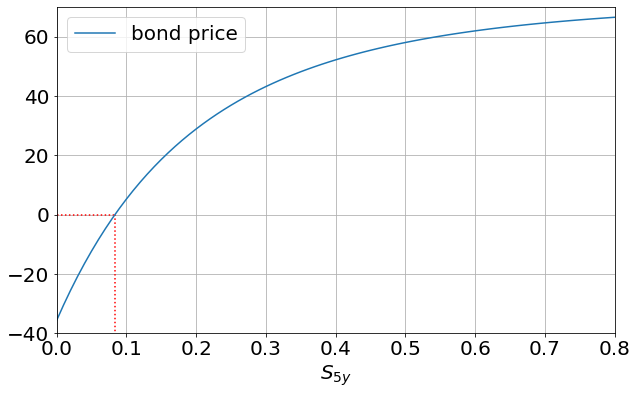
\includegraphics[width=0.7\textwidth]{figures/bond_5_plot.png}
  \caption{Plot of the discounted cash flow of bond 5 as a function of the 5 year spot rate.}
  \label{fig:fifth_year_rate}
\end{figure}

\begin{tcolorbox}[breakable, size=fbox, boxrule=1pt, pad at break*=1mm,colback=cellbackground, colframe=cellborder]
\begin{Verbatim}[commandchars=\\\{\}]
\PY{k+kn}{from} \PY{n+nn}{scipy}\PY{n+nn}{.}\PY{n+nn}{optimize} \PY{k}{import} \PY{n}{brentq}

\PY{k}{def} \PY{n+nf}{func}\PY{p}{(}\PY{n}{x}\PY{p}{)}\PY{p}{:}
    \PY{k}{return} \PY{l+m+mi}{100} \PY{o}{\PYZhy{}} \PY{l+m+mi}{8}\PY{o}{/}\PY{p}{(}\PY{l+m+mi}{1}\PY{o}{+}\PY{l+m+mf}{0.04}\PY{p}{)} \PY{o}{\PYZhy{}} \PY{l+m+mi}{8}\PY{o}{/}\PY{p}{(}\PY{l+m+mi}{1}\PY{o}{+}\PY{l+m+mf}{0.0503}\PY{p}{)}\PY{o}{*}\PY{o}{*}\PY{l+m+mi}{2} \PY{o}{\PYZhy{}} \PY{l+m+mi}{8}\PY{o}{/}\PY{p}{(}\PY{l+m+mi}{1}\PY{o}{+}\PY{l+m+mf}{0.0608}\PY{p}{)}\PY{o}{*}\PY{o}{*}\PY{l+m+mi}{3} 
               \PY{o}{\PYZhy{}} \PY{l+m+mi}{8}\PY{o}{/}\PY{p}{(}\PY{l+m+mi}{1}\PY{o}{+}\PY{l+m+mf}{0.0719}\PY{p}{)}\PY{o}{*}\PY{o}{*}\PY{l+m+mi}{4} \PY{o}{\PYZhy{}} \PY{l+m+mi}{108}\PY{o}{/}\PY{p}{(}\PY{l+m+mi}{1}\PY{o}{+}\PY{n}{x}\PY{p}{)}\PY{o}{*}\PY{o}{*}\PY{l+m+mi}{5}

\PY{n}{a} \PY{o}{=} \PY{n}{brentq}\PY{p}{(}\PY{n}{func}\PY{p}{,} \PY{l+m+mi}{0}\PY{p}{,} \PY{l+m+mf}{0.10}\PY{p}{)}
\PY{n+nb}{print} \PY{p}{(}\PY{l+s+s2}{\PYZdq{}}\PY{l+s+s2}{5y rate: }\PY{l+s+si}{\PYZob{}:.4f\PYZcb{}}\PY{l+s+s2}{\PYZdq{}}\PY{o}{.}\PY{n}{format}\PY{p}{(}\PY{n}{a}\PY{p}{)}\PY{p}{)}

5y rate: 0.0836
\end{Verbatim}
\end{tcolorbox}

The very same mechanism can be generalized and extended to more maturities to get a more detailed yield curve. In general terms the previous system becomes

\begin{equation}
\begin{cases}
f_1(S_1, p_1) = 0 \\
f_2(S_1, S_2, p_2) = 0 \\
f_3(S_1, S_2, S_3, p_3) = 0 \\
f_4(S_1, S_2, S_3, S_4, p_4) = 0 \\
\cdots
\end{cases}
\end{equation}
where $S_i$ are the unknown spot rates and $p_i$ the market quotes of the considered products. The iterative procedure we have applied before exploits the first equation to find $S_1 = f_1^{-1}(p_1)$, the second to find $S_2 = f_2^{-1}(S_1, p_2)$ and so on and so forth; this algorithm works since each equation will determine exactly one \emph{free} spot rate which is not already determined by the others.

\subsection{Bootstrapping as Minimization Problem}
We can now describe the bootstrap algorithm in general terms as follows:
\begin{enumerate}
\item define a set of yielding products (e.g. coupon-bearing bonds, swaps);
%\item derive discount factors for the corresponding terms;
\item \emph{bootstrap} the zero-coupon curve, successively calibrating it such that it returns the market quotes of these inputs.
\end{enumerate}

Instead of iteratively finding the solution of each equation as before, we could define a vector of spot rates $\mathbf{S} = (S_1, S_2, S_3, \ldots)$ seeking for a particular $\mathbf{\hat{S}}$ which solves the following equation:

\begin{equation}
F = f_1^2(\hat{S}_1) + f_2^2(\hat{S}_1, \hat{S}_2) + f_3^2(\hat{S}_1, \hat{S}_2, \hat{S}_3) + f_4^2(\hat{S}_1, \hat{S}_2, \hat{S}_3, \hat{S}_4) + \ldots = 0
\end{equation}

Under this terms the bootstrap method can be considered as a minimization algorithm, indeed we need to find $\mathbf{\hat{S}}$ which \emph{minimize} $F$, or makes it as close as possible to 0.
Notice how each \(f_i\) is squared since we want all of them to be minimized at the same time and not only \(F\) globally (i.e. without the square there may be cancellation effects between the terms of the sum).

\subsection{Minimization Algorithm}\label{minimization-algorithm}

A minimization algorithm follows these steps:

\begin{itemize}
\tightlist
\item
  define an \emph{objective function} i.e. the function that has to be
  minimized to reach our goal;
\item
  set the initial value of the unknown parameters (\(\mathbf{x_0}\)) and their range of
  variability;
\item
  the minimizer computes the objective function value;
\item
  then it moves the parameter values in such a way to find a smaller
  value of the objective function (e.g. following the direction derivative w.r.t.
  each parameter);
\item if constraints are defined, they will be considered in the previous step;
\item
  the last three steps will be repeated until further variations of the
  \(\mathbf{x}\) values won't change significantly the objective
  function (i.e. we have found a minimum of the function so the
  minimization process is completed !).
\end{itemize}

Let's see with a couple of example how minimization can be implemented in \texttt{python} using the function \texttt{scipy.optimize.minimize}.

\subsubsection{A Simple Minimization Example}
\label{example}

Find the size of a circular cylindrical can of volume, \(330~\mathrm{cm}^3\),
that minimizes the cost of manufacture, see Figure~\ref{fig:cylinder}.

\begin{figure}[h]
\centering
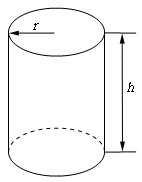
\includegraphics[width=0.2\textwidth]{figures/cylinder.png}
\caption{Graphical representation of the \emph{can} minimization example.}
\label{fig:cylinder}
\end{figure}

Clearly to minimize the costs, the company needs to reduce the can
surface

\begin{equation*} 
S = 2\pi rh + 2\cdot(\pi r^2) 
\end{equation*}
On the other hand the volume is fixed to \(330~\mathrm{cm}^3\) so previous
equation can be simplified by removing \(h\)

\begin{equation*} 
V = \pi r^2 h = 330\quad\implies h = \cfrac{330}{\pi r^2}
\end{equation*}
In the end the function to be minimized is

\begin{equation}
S = 2\pi rh + 2\cdot(\pi r^2) = \cfrac{2\cdot 330}{r} + 2\cdot(\pi r^2)
\end{equation}
This is the objective function, and the parameter set is represented 
by \(\tt{x[0]}\) which is the can radius.

\begin{tcolorbox}[breakable, size=fbox, boxrule=1pt, pad at break*=1mm,colback=cellbackground, colframe=cellborder]
\begin{Verbatim}[commandchars=\\\{\}]
\PY{k+kn}{from} \PY{n+nn}{math} \PY{k}{import} \PY{n}{pi}

\PY{k}{def} \PY{n+nf}{obj_func}\PY{p}{(}\PY{n}{x}\PY{p}{)}\PY{p}{:}
    \PY{k}{return} \PY{l+m+mi}{2}\PY{o}{*}\PY{l+m+mi}{330}\PY{o}{/}\PY{n}{x}\PY{p}{[}\PY{l+m+mi}{0}\PY{p}{]} \PY{o}{+} \PY{l+m+mi}{2}\PY{o}{*}\PY{n}{pi}\PY{o}{*}\PY{n}{x}\PY{p}{[}\PY{l+m+mi}{0}\PY{p}{]}\PY{o}{*}\PY{o}{*}\PY{l+m+mi}{2}
\end{Verbatim}
\end{tcolorbox}
\noindent
Set the limits to our unknown variable and its initial value:

\begin{tcolorbox}[breakable, size=fbox, boxrule=1pt, pad at break*=1mm,colback=cellbackground, colframe=cellborder]
\begin{Verbatim}[commandchars=\\\{\}]
\PY{n}{x0} \PY{o}{=} \PY{p}{[}\PY{l+m+mi}{1}\PY{p}{]}
\PY{n}{bounds} \PY{o}{=} \PY{p}{[}\PY{p}{(}\PY{l+m+mf}{0.01}\PY{p}{,} \PY{l+m+mi}{100}\PY{p}{)}\PY{p}{]}
\end{Verbatim}
\end{tcolorbox}
\noindent
Finally we run the minimization:

\begin{tcolorbox}[breakable, size=fbox, boxrule=1pt, pad at break*=1mm,colback=cellbackground, colframe=cellborder]
\begin{Verbatim}[commandchars=\\\{\}]
\PY{n}{r} \PY{o}{=} \PY{n}{minimize}\PY{p}{(}\PY{n}{obj_func}\PY{p}{,} \PY{n}{x0}\PY{p}{,} \PY{n}{bounds}\PY{o}{=}\PY{n}{bounds}\PY{p}{)}
\PY{n+nb}{print} \PY{p}{(}\PY{n}{r}\PY{p}{)}

      fun: 264.356810914805
 hess\_inv: <1x1 LbfgsInvHessProduct with dtype=float64>
      jac: array([5.68434189e-06])
  message: b'CONVERGENCE: NORM\_OF\_PROJECTED\_GRADIENT\_<=\_PGTOL'
     nfev: 24
      nit: 9
   status: 0
  success: True
        x: array([3.7449385])
    \end{Verbatim}
\end{tcolorbox}

So to minimize the cost the company should produce cans with a radius of
about 3.745 cm (I suspect that Coke have done a similar calculation since the result is quite close to a real can).

\subsubsection{Another Example with Constraint}
\label{example-with-constraint}

We are going to fence a rectangular field. If we look at the field
from above the cost of the vertical sides are \$10/m, the cost of the
bottom is \$2/m and the cost of the top side is \$7/m. If we have a \$700 budget determine
the dimensions of the field that will maximize the enclosed area, see Fig.~\ref{fig:field}.

\begin{figure}[h]
\centering
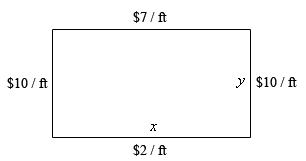
\includegraphics[width=0.4\textwidth]{figures/field.png}
\caption{Graphical representation of the \emph{field} minimization example.}
\label{fig:field}
\end{figure}

In this example there are two differences with respect to the previous one:

\begin{itemize}
\tightlist
\item
  we want to \emph{maximize} a quantity (not minimize);
\item
  there is a constraint (we have a limited budget).
\end{itemize}

So let's repeat the steps as before. The objective is to maximize the
enclosed area \(A\) but our algorithm can only minimize; we can define the objective function 
to return the quantity \(-A\), so that if we minimize it at the same time 
we are maximizing our real objective, $A$. 
Define length and width of the field respectively as \(\tt{x[0]}\) and
\(\tt{x[1]}\) (items of the list \texttt{x}):

\begin{tcolorbox}[breakable, size=fbox, boxrule=1pt, pad at break*=1mm,colback=cellbackground, colframe=cellborder]
\begin{Verbatim}[commandchars=\\\{\}]
\PY{k}{def} \PY{n+nf}{of}\PY{p}{(}\PY{n}{x}\PY{p}{)}\PY{p}{:}
    \PY{k}{return} \PY{o}{\PYZhy{}}\PY{n}{x}\PY{p}{[}\PY{l+m+mi}{0}\PY{p}{]}\PY{o}{*}\PY{n}{x}\PY{p}{[}\PY{l+m+mi}{1}\PY{p}{]}
\end{Verbatim}
\end{tcolorbox}
\noindent
We can set the boundaries for length and width with their initial values (1~m each):

\begin{tcolorbox}[breakable, size=fbox, boxrule=1pt, pad at break*=1mm,colback=cellbackground, colframe=cellborder]
\begin{Verbatim}[commandchars=\\\{\}]
\PY{n}{x0} \PY{o}{=} \PY{p}{[}\PY{l+m+mi}{1}\PY{p}{,} \PY{l+m+mi}{1}\PY{p}{]}
\PY{n}{bounds} \PY{o}{=} \PY{p}{[}\PY{p}{(}\PY{l+m+mf}{0.01}\PY{p}{,} \PY{l+m+mi}{100}\PY{p}{)} \PY{k}{for} \PY{n}{\PYZus{}} \PY{o+ow}{in} \PY{n+nb}{range}\PY{p}{(}\PY{n+nb}{len}\PY{p}{(}\PY{n}{x0}\PY{p}{)}\PY{p}{)}\PY{p}{]}
\end{Verbatim}
\end{tcolorbox}

Finally we have to impose the constraint on the money. This is done by
defining a function that computes the money spent with the fence and
compare it to \$700. The constraint is passed to the minimizer with a
dictionary which has two keys: \(\tt{type}\), in this case set to \texttt{'eq'}
(like equality, since we want to spend all of our available money so the
fence has to cost equal to \$700) and \texttt{'fun'} which defines the constraint 
function which for this example implements a calculation like

\begin{equation*}
\begin{gathered}
\mathrm{fence~cost} = l\cdot10 + l\cdot10 + w\cdot2 + w\cdot7 = 700\\
700 - l\cdot10 - l\cdot10 - w\cdot2 - w\cdot7 = 0
\end{gathered}
\end{equation*}

\begin{tcolorbox}[breakable, size=fbox, boxrule=1pt, pad at break*=1mm,colback=cellbackground, colframe=cellborder]
\begin{Verbatim}[commandchars=\\\{\}]
\PY{k}{def} \PY{n+nf}{cons}\PY{p}{(}\PY{n}{x}\PY{p}{)}\PY{p}{:}
    \PY{k}{return} \PY{l+m+mi}{700} \PY{o}{\PYZhy{}} \PY{n}{x}\PY{p}{[}\PY{l+m+mi}{0}\PY{p}{]}\PY{o}{*}\PY{l+m+mi}{20} \PY{o}{\PYZhy{}} \PY{n}{x}\PY{p}{[}\PY{l+m+mi}{1}\PY{p}{]}\PY{o}{*}\PY{l+m+mi}{2} \PY{o}{\PYZhy{}} \PY{n}{x}\PY{p}{[}\PY{l+m+mi}{1}\PY{p}{]}\PY{o}{*}\PY{l+m+mi}{7}

\PY{n}{constraints} \PY{o}{=} \PY{p}{\PYZob{}}\PY{l+s+s1}{\PYZsq{}}\PY{l+s+s1}{type}\PY{l+s+s1}{\PYZsq{}}\PY{p}{:}\PY{l+s+s1}{\PYZsq{}}\PY{l+s+s1}{eq}\PY{l+s+s1}{\PYZsq{}}\PY{p}{,} \PY{l+s+s1}{\PYZsq{}}\PY{l+s+s1}{fun}\PY{l+s+s1}{\PYZsq{}}\PY{p}{:}\PY{n}{cons}\PY{p}{\PYZcb{}}
\end{Verbatim}
\end{tcolorbox}
\noindent
Now we can call the minimizer.

\begin{tcolorbox}[breakable, size=fbox, boxrule=1pt, pad at break*=1mm,colback=cellbackground, colframe=cellborder]
\begin{Verbatim}[commandchars=\\\{\}]
\PY{n}{r} \PY{o}{=} \PY{n}{minimize}\PY{p}{(}\PY{n}{of}\PY{p}{,} \PY{n}{x0}\PY{p}{,} \PY{n}{bounds}\PY{o}{=}\PY{n}{bounds}\PY{p}{,} \PY{n}{constraints}\PY{o}{=}\PY{n}{constraints}\PY{p}{)}
\PY{n+nb}{print} \PY{p}{(}\PY{n}{r}\PY{p}{)}

     fun: -680.5555555555482
     jac: array([-38.88889313, -17.5       ])
 message: 'Optimization terminated successfully.'
    nfev: 16
     nit: 4
    njev: 4
  status: 0
 success: True
       x: array([17.49999818, 38.88889293])
    \end{Verbatim}
\end{tcolorbox}

So the field will come out \(17.5\)~m long and \(38.9\)~m wide.

\subsection{Local Minima}
When the objective function has local minima the choice of the initial value of the parameters can be critical. 
Assume we would like to minimize an objective function like 

\[
f(x) = \cfrac{\mathrm{cos}(3\pi x)}{x}
\]
This function is plotted in Fig.~\ref{fig:local_minima} in the range $[0, 2]$, and it is clear that it has many minima. 

\begin{figure}[htb]
	\centering
	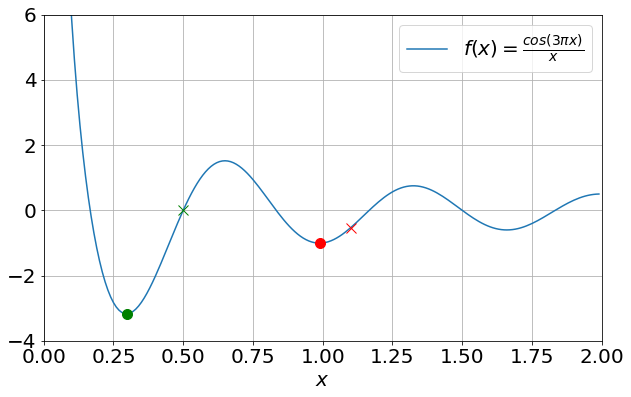
\includegraphics[width=0.7\textwidth]{figures/local_minima.png}
	\caption{Plot of an example function with many local minima. The red points highlights initial value and minimum found in a \emph{bad} minimization, green points for a good minimization.}
	\label{fig:local_minima}
\end{figure}

Let's try to find a minimum and set the initial value to $x=1.1$.
\begin{tcolorbox}[breakable, size=fbox, boxrule=1pt, pad at break*=1mm,colback=cellbackground, colframe=cellborder]
\begin{Verbatim}[commandchars=\\\{\}]
\PY{k+kn}{from} \PY{n+nn}{scipy}\PY{n+nn}{.}\PY{n+nn}{optimize} \PY{k}{import} \PY{n}{minimize}
\PY{n}{x0} \PY{o}{=} \PY{p}{[}\PY{l+m+mf}{1.1}\PY{p}{]}
\PY{n}{bounds} \PY{o}{=} \PY{p}{[}\PY{p}{(}\PY{l+m+mf}{0.01}\PY{p}{,} \PY{l+m+mi}{20}\PY{p}{)}\PY{p}{]}
		
\PY{n}{r} \PY{o}{=} \PY{n}{minimize}\PY{p}{(}\PY{n}{func}\PY{p}{,} \PY{n}{x0}\PY{p}{,} \PY{n}{bounds}\PY{o}{=}\PY{n}{bounds}\PY{p}{)}
\PY{n+nb}{print} \PY{p}{(}\PY{n}{r}\PY{p}{)}

     fun: array([-1.00569871])
hess\_inv: <1x1 LbfgsInvHessProduct with dtype=float64>
     jac: array([-4.4408921e-07])
 message: b'CONVERGENCE: NORM\_OF\_PROJECTED\_GRADIENT\_<=\_PGTOL'
    nfev: 16
     nit: 5
  status: 0
 success: True
       x: array([0.98865633])
\end{Verbatim}
\end{tcolorbox}
The minimization worked perfectly and we found $x=0.98865633$ (i.e. the red point in Fig.~\ref{fig:local_minima}) but still from the same Figure it is clear that this is not the absolute minimum we wanted to find. The problem arise since the algorithm has got stuck in a local minimum without any possibility to jump out from the well.

If we repeat the minimization using as initial value $0.5$ instead
\begin{tcolorbox}[breakable, size=fbox, boxrule=1pt, pad at break*=1mm,colback=cellbackground, colframe=cellborder]
\begin{Verbatim}[commandchars=\\\{\}]
\PY{k+kn}{from} \PY{n+nn}{scipy}\PY{n+nn}{.}\PY{n+nn}{optimize} \PY{k}{import} \PY{n}{minimize}
\PY{n}{x0} \PY{o}{=} \PY{p}{[}\PY{l+m+mf}{0.5}\PY{p}{]}
\PY{n}{bounds} \PY{o}{=} \PY{p}{[}\PY{p}{(}\PY{l+m+mf}{0.01}\PY{p}{,} \PY{l+m+mi}{20}\PY{p}{)}\PY{p}{]}
		
\PY{n}{r} \PY{o}{=} \PY{n}{minimize}\PY{p}{(}\PY{n}{func}\PY{p}{,} \PY{n}{x0}\PY{p}{,} \PY{n}{bounds}\PY{o}{=}\PY{n}{bounds}\PY{p}{)}
\PY{n+nb}{print} \PY{p}{(}\PY{n}{r}\PY{p}{)}

     fun: array([-3.17151711])
hess\_inv: <1x1 LbfgsInvHessProduct with dtype=float64>
     jac: array([9.76996262e-07])
 message: b'CONVERGENCE: NORM\_OF\_PROJECTED\_GRADIENT\_<=\_PGTOL'
    nfev: 16
     nit: 5
  status: 0
 success: True
       x: array([0.29691798])
\end{Verbatim}
\end{tcolorbox}
Now clearly the algorithm found the absolute minimum in $x=0.29691798$ (i.e. the green point in Fig.~\ref{fig:local_minima}) because there was no chance to find a local minimum during the iterations.

This is just an example of what could happen when minimizing a function.
When dealing with complicated cases it is possible to make a \emph{scan} of the objective 
function to try to approximately determine where the global minimum is and choose 
suitable initial values of the guess parameters.
There shouldn't be such an issue in the application of the bootstrap algorithm though since the function that we are going to minimize is a sum of squared terms which has no local minima, just a global minimum (i.e. it is a hyper-parabola).

\subsection{Back to OIS Example}\label{ois-example}
The general idea here is to get the discount curve \(\mathcal{C}\) that prices correctly 
each OIS by minimizing the sum of their NPV squared (our \(f_i\)):

\begin{equation}
\mathrm{min}_{\mathcal{C}} \Big\{\sum_{i=1}^{n}\mathrm{NPV}(\mathrm{OIS}_i, \mathcal{C})^2\Big\}
\end{equation}

A discount curve is characterized by pillar dates and discount factors. The description of the problem we have given above does not, specifies any constraint on the number of pillar dates of 
the discount curve \(\mathcal{C}\). However, the pillar dates determine the number of unknown variables of the optimization problem. A curve with \(N\) pillar dates has \(N\) discount factors (note that the first discount factor, with value date equal to the today date, is constrained to 1). \textbf{In practice, therefore, it makes sense to choose the pillar dates in such a way that 
	there are exactly the right number of degrees of freedom in the optimization to match data.} 
The natural choice is to choose the pillar dates of the discount curve equal to the set of expiry dates of the swaps.

Once we've fixed \(\mathbf{d}\) to be a vector of pillar dates equal to the expiry dates of the swaps, and we use \(\mathbf{x}\) to represent the vector of discount factors, then the problem becomes:

\begin{equation}
\mathrm{min}_{\mathbf{x}} \Big\{\sum_{i=1}^{N}\mathrm{NPV}(\mathrm{OIS}_i, \mathcal{C}(\mathbf{d}, \mathbf{x}))^2\Big\}
\end{equation}
which is our optimization problem: (\textbf{to find the minimum of the above expression as a function of x}) that can be solved using one of the available numerical optimization routines 
in \texttt{python}.

So first let's create the swaps according to all the available market
quotes and also the pillar dates of our final discount curve:

\begin{tcolorbox}[breakable, size=fbox, boxrule=1pt, pad at break*=1mm,colback=cellbackground, colframe=cellborder]
\begin{Verbatim}[commandchars=\\\{\}]
\PY{k+kn}{from} \PY{n+nn}{finmarkets} \PY{k}{import} \PY{n}{generate\PYZus{}swap\PYZus{}dates}

\PY{n}{observation\PYZus{}date} \PY{o}{=} \PY{n}{date}\PY{p}{(}\PY{l+m+mi}{2019}\PY{p}{,} \PY{l+m+mi}{10}\PY{p}{,} \PY{l+m+mi}{23}\PY{p}{)}
\PY{n}{pillar\PYZus{}dates} \PY{o}{=} \PY{p}{[}\PY{n}{observation\PYZus{}date}\PY{p}{]}
\PY{n}{swaps} \PY{o}{=} \PY{p}{[}\PY{p}{]} 

\PY{k}{for} \PY{n}{i} \PY{o+ow}{in} \PY{n+nb}{range}\PY{p}{(}\PY{n+nb}{len}\PY{p}{(}\PY{n}{df}\PY{p}{)}\PY{p}{)}\PY{p}{:}
    \PY{n}{swap} \PY{o}{=} \PY{n}{OvernightIndexSwap}\PY{p}{(}\PY{l+m+mf}{1e6}\PY{p}{,}
                    \PY{n}{generate\PYZus{}swap\PYZus{}dates}\PY{p}{(}\PY{n}{observation\PYZus{}date}\PY{p}{,}  
                                        \PY{n}{mq}\PY{p}{[}\PY{l+s+s1}{\PYZsq{}}\PY{l+s+s1}{months}\PY{l+s+s1}{\PYZsq{}}\PY{p}{]}\PY{o}{.}\PY{n}{tolist}\PY{p}{(}\PY{p}{)}\PY{p}{[}\PY{n}{i}\PY{p}{]}\PY{p}{)}\PY{p}{,}
                    \PY{l+m+mf}{0.01} \PY{o}{*} \PY{n}{mq}\PY{p}{[}\PY{l+s+s1}{\PYZsq{}}\PY{l+s+s1}{quote}\PY{l+s+s1}{\PYZsq{}}\PY{p}{]}\PY{o}{.}\PY{n}{tolist}\PY{p}{(}\PY{p}{)}\PY{p}{[}\PY{n}{i}\PY{p}{]}\PY{p}{)}
    \PY{n}{swaps}\PY{o}{.}\PY{n}{append}\PY{p}{(}\PY{n}{swap}\PY{p}{)}
    \PY{n}{pillar\PYZus{}dates}\PY{o}{.}\PY{n}{append}\PY{p}{(}\PY{n}{swap}\PY{o}{.}\PY{n}{payment\PYZus{}dates}\PY{p}{[}\PY{o}{\PYZhy{}}\PY{l+m+mi}{1}\PY{p}{]}\PY{p}{)}

\PY{n}{pillar\PYZus{}dates} \PY{o}{=} \PY{n+nb}{sorted}\PY{p}{(}\PY{n}{pillar\PYZus{}dates}\PY{p}{)}
\end{Verbatim}
\end{tcolorbox}

So let's review step by step the implementation of the bootstrapping just described.

\begin{itemize}
\tightlist
\item
  define the objective function: the sum of the squared NPVs of the OIS

\begin{tcolorbox}[breakable, size=fbox, boxrule=1pt, pad at break*=1mm,colback=cellbackground, colframe=cellborder]
\begin{Verbatim}[commandchars=\\\{\}]
\PY{k}{import} \PY{n+nn}{numpy} \PY{k}{as} \PY{n}{np}

\PY{k}{def} \PY{n+nf}{objective\PYZus{}function}\PY{p}{(}\PY{n}{x}\PY{p}{)}\PY{p}{:}
    \PY{n}{x = np.insert(x, 0, 1)}
    \PY{n}{curve} \PY{o}{=} \PY{n}{DiscountCurve}\PY{p}{(}\PY{n}{observation\PYZus{}date}\PY{p}{,} \PY{n}{pillar\PYZus{}dates}\PY{p}{,} \PY{n}{x}\PY{p}{)}
    
    \PY{n}{sum\PYZus{}sq} \PY{o}{=} \PY{l+m+mf}{0.0}
    \PY{k}{for} \PY{n}{swap} \PY{o+ow}{in} \PY{n}{swaps}\PY{p}{:}
        \PY{n}{sum\PYZus{}sq} \PY{o}{+}\PY{o}{=} \PY{n}{swap}\PY{o}{.}\PY{n}{npv}\PY{p}{(}\PY{n}{curve}\PY{p}{)} \PY{o}{*}\PY{o}{*} \PY{l+m+mi}{2}
    \PY{k}{return} \PY{n}{sum\PYZus{}sq}
\end{Verbatim}
\end{tcolorbox}

\item
  set the initial value of the discount factors (\(x_i^0\)) to 1 with a
  range of variability \([ 0.01, 10]\), today's discount factor is not considered 
  in the list since it is fixed to 1 but is added explicitly in the objective function
  for the calculation of the NPV's (see \texttt{insert} command)

\begin{tcolorbox}[breakable, size=fbox, boxrule=1pt, pad at break*=1mm,colback=cellbackground, colframe=cellborder]
\begin{Verbatim}[commandchars=\\\{\}]
\PY{n}{x0} \PY{o}{=} \PY{p}{[}\PY{l+m+mf}{1.0} \PY{k}{for} \PY{n}{i} \PY{o+ow}{in} \PY{n+nb}{range}\PY{p}{(}\PY{n+nb}{len}\PY{p}{(}\PY{n}{pillar\PYZus{}dates}\PY{p}{)-1}\PY{p}{)}\PY{p}{]}
\PY{n}{bounds} \PY{o}{=} \PY{p}{[}\PY{p}{(}\PY{l+m+mf}{0.01}\PY{p}{,} \PY{l+m+mf}{10.0}\PY{p}{)} \PY{k}{for} \PY{n}{i} \PY{o+ow}{in} \PY{n+nb}{range}\PY{p}{(}\PY{n+nb}{len}\PY{p}{(}\PY{n}{pillar\PYZus{}dates}\PY{p}{)-1}\PY{p}{)}\PY{p}{]}
\end{Verbatim}
\end{tcolorbox}

\item
  finally we can launch the minimizer to find the discount factors
  (\(\mathbf{x}\))

\begin{tcolorbox}[breakable, size=fbox, boxrule=1pt, pad at break*=1mm,colback=cellbackground, colframe=cellborder]
\begin{Verbatim}[commandchars=\\\{\}]
\PY{k+kn}{from} \PY{n+nn}{scipy}\PY{n+nn}{.}\PY{n+nn}{optimize} \PY{k}{import} \PY{n}{minimize}

\PY{n}{result} \PY{o}{=} \PY{n}{minimize}\PY{p}{(}\PY{n}{objective\PYZus{}function}\PY{p}{,} \PY{n}{x0}\PY{p}{,} \PY{n}{bounds}\PY{o}{=}\PY{n}{bounds}\PY{p}{)}
\PY{n+nb}{print} \PY{p}{(}\PY{n}{result}\PY{p}{)}
\end{Verbatim}
\end{tcolorbox}

\begin{Verbatim}[commandchars=\\\{\}]
      fun: 0.000819919032900304
 hess\_inv: <34x34 LbfgsInvHessProduct with dtype=float64>
      jac: array([ 6.58948735e+05, -1.58720803e+01, -6.53143264e+01,
-1.03323232e+02,
       -1.26050260e+02, -1.31748898e+02, -1.20374599e+02, -9.15399651e+01,
       -4.24363322e+01,  2.44903182e+01,  1.14345243e+02,  2.22002243e+02,
       -3.72021700e+00,  4.21398633e+01,  4.21787852e+01,  4.22369487e+01,
        4.23327026e+01,  4.31814758e+01,  4.44924460e+01,  4.62078978e+01,
        4.82906823e+01, -3.69972738e+00, -1.42454702e+00,  7.53771932e-01,
        2.79741018e+00,  4.62896699e+00,  6.24844054e+00,  9.93101553e+00,
        1.31122434e+01,  1.42880909e+01,  1.48279215e+01,  1.50787019e+01,
        1.43267935e+01,  1.38451324e+01])
  message: b'CONVERGENCE: REL\_REDUCTION\_OF\_F\_<=\_FACTR*EPSMCH'
     nfev: 840
      nit: 7
   status: 0
  success: True
        x: array([1.        , 1.00030147, 1.00058831, 1.00089012, 1.00119726,
                  1.00147996, 1.00178743, 1.00208107, 1.00238467, 1.00267865,
                  1.00298261, 1.00327737, 1.00357104, 1.00357104, 1.00355063,
                  1.00352002, 1.00346901, 1.00302007, 1.00232627, 1.00141821,
                  1.00031629, 0.99911234, 0.99790839, 0.99675545, 0.99567393,
                  0.99470465, 0.9938476 , 0.99189884, 0.99021534, 0.98959296,
                  0.98930728, 0.98917464, 0.98957256, 0.98982763])
\end{Verbatim}
\end{itemize}

Printing the result gives us the a lot of information about the minimisation just performed, the most useful are:
\begin{itemize}
\item \texttt{func}: the value of the objective function at the last iteration;
\item \texttt{message}: the summary message from the algorithm (if it is \texttt{CONVERGENCE} is almost always OK);
\item \texttt{success}: the name is self explanatory;
\item \texttt{x}: the vector of unknown parameters that have been optimised.
\end{itemize}

Another useful check to perform in order to understand if everything went fine, is the comparison of the objective function with the initial guessed parameters and at the end of the minimisation.

\begin{tcolorbox}[breakable, size=fbox, boxrule=1pt, pad at break*=1mm,colback=cellbackground, colframe=cellborder]
\begin{Verbatim}[commandchars=\\\{\}]
\PY{n+nb}{print} \PY{p}{(}\PY{l+s+s2}{\PYZdq{}}\PY{l+s+s2}{Initial objective function value }\PY{l+s+s2}{\PYZdq{}}\PY{p}{,} \PY{n}{objective\PYZus{}function}\PY{p}{(}\PY{n}{x0}\PY{p}{)}\PY{p}{)}
\PY{n+nb}{print} \PY{p}{(}\PY{l+s+s2}{\PYZdq{}}\PY{l+s+s2}{Final objective function value }\PY{l+s+s2}{\PYZdq{}}\PY{p}{,} \PY{n}{objective\PYZus{}function}\PY{p}{(}\PY{n}{result}\PY{o}{.}\PY{n}{x}\PY{p}{)}\PY{p}{)}
	
Initial objective function value  26.27213544937082
Final objective function value  5.664309920943246e-11
\end{Verbatim}
\end{tcolorbox}
The objective function at the end of the minimisation is not exactly 0 (and rarely it will be) but its value is small enough for us to be satisfied, we started with $30$ and now it is $10^{-11}$ so 13 orders of magnitude smaller. This means that with the derived discount curve the NPV's of our OIS won't be identically 0 but so small that we can consider them as they were.

It can be very useful to also look at some diagnostic plots to check if the minimization was successful. Figure~\ref{fig:minimization_diagnostic} reports on the left the objective function value as a function of discount factor $(x_0)$; clearly we have found a minimum (the orange point represent $x_0$ value at the end of the minimization). On the right instead, the value of the objective function at each iteration is shown, its value is decreasing dramatically (notice that the $y$ axis is drawn in log scale).

\begin{figure}[htb]
	\centering
	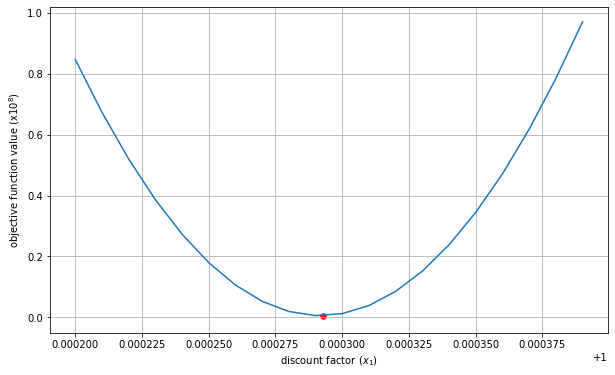
\includegraphics[width=0.45\linewidth]{figures/obj_func.png}
	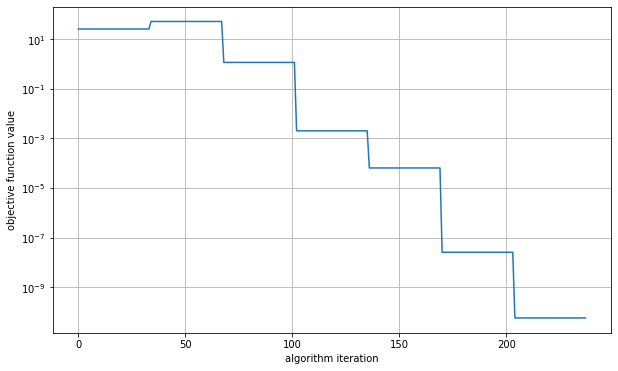
\includegraphics[width=0.45\linewidth]{figures/obj_func_iter.png}
	\caption{Diagnostic plots for the minimization algorithm. On the left the objective function value as a function of the discount factor $x_0$, on the right the objective function value as a function of the iteration number (the orange point represent $x_0$ value at the end of the minimization).}
	\label{fig:minimization_diagnostic}
\end{figure}

Finally we can create the discount curve implied by the market quotes of
our swaps (see Fig.~\ref{fig:discount_curve}) and try to compute some implied rates.

\begin{tcolorbox}[breakable, size=fbox, boxrule=1pt, pad at break*=1mm,colback=cellbackground, colframe=cellborder]
\begin{Verbatim}[commandchars=\\\{\}]
\PY{k+kn}{from} \PY{n+nn}{math} \PY{k}{import} \PY{n}{log}
	
\PY{n}{dfs} \PY{o}{=} \PY{n}{np}\PY{o}{.}\PY{n}{insert}\PY{p}{(}\PY{n}{result}\PY{o}{.}\PY{n}{x}\PY{p}{,} \PY{l+m+mi}{0}\PY{p}{,} \PY{l+m+mi}{1}\PY{p}{)}
\PY{n}{curve} \PY{o}{=} \PY{n}{DiscountCurve}\PY{p}{(}\PY{n}{observation\PYZus{}date}\PY{p}{,} \PY{n}{pillar\PYZus{}dates}\PY{p}{,} \PY{n}{dfs}\PY{p}{)}
	
\PY{n}{d} \PY{o}{=} \PY{n}{date}\PY{p}{(}\PY{l+m+mi}{2059}\PY{p}{,} \PY{l+m+mi}{11}\PY{p}{,} \PY{l+m+mi}{23}\PY{p}{)}
\PY{n+nb}{print} \PY{p}{(}\PY{l+s+s2}{\PYZdq{}}\PY{l+s+s2}{40y df: }\PY{l+s+si}{\PYZob{}\PYZcb{}}\PY{l+s+s2}{\PYZdq{}}\PY{o}{.}\PY{n}{format}\PY{p}{(}\PY{n}{curve}\PY{o}{.}\PY{n}{df}\PY{p}{(}\PY{n}{d}\PY{p}{)}\PY{p}{)}\PY{p}{)}
\PY{n+nb}{print} \PY{p}{(}\PY{l+s+s2}{\PYZdq{}}\PY{l+s+s2}{40y rate: }\PY{l+s+si}{\PYZob{}\PYZcb{}}\PY{l+s+s2}{\PYZdq{}}\PY{o}{.}\PY{n}{format}\PY{p}{(}\PY{o}{\PYZhy{}}\PY{n}{log}\PY{p}{(}\PY{n}{curve}\PY{o}{.}\PY{n}{df}\PY{p}{(}\PY{n}{d}\PY{p}{)}\PY{p}{)} \PY{o}{/} \PY{l+m+mi}{40}\PY{p}{)}\PY{p}{)}             
	
40y df: 0.6454865298509954
40y rate: 0.01094377341721375
\end{Verbatim}
\end{tcolorbox}

\begin{figure}[htb]
	\centering
	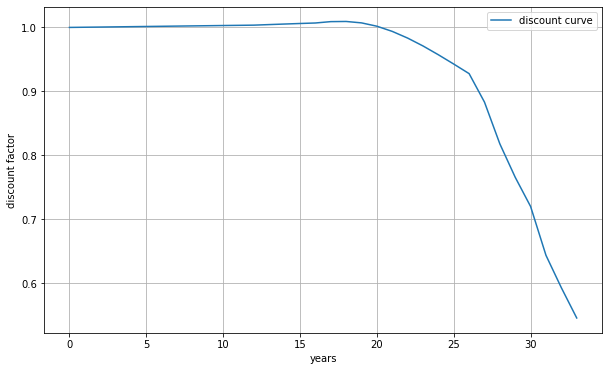
\includegraphics[width=0.7\textwidth]{figures/example_discount_curve.png}
	\caption{Plot of the discount curve implied by Overnight Index Swap market quotes.}
	\label{fig:discount_curve}
\end{figure}

\begin{thebibliography}{9}
	\bibitem{bib:bootsrap} \href{https://financetrain.com/bootstrapping-spot-rate-curve-zero-curve}{\emph{Bootstrapping Spot Rate Curve}} [Online]
\end{thebibliography}
